% Created by tikzDevice version 0.12.3.1 on 2022-02-12 21:52:23
% !TEX encoding = UTF-8 Unicode
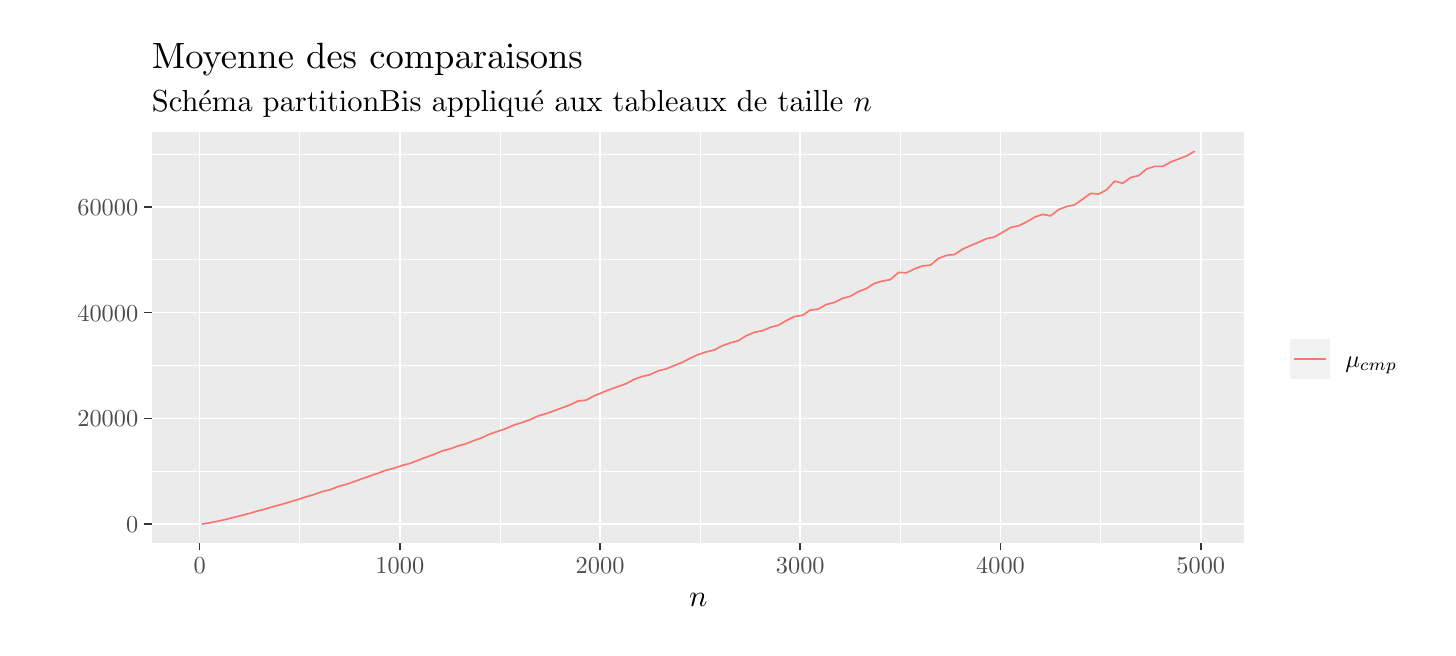
\begin{tikzpicture}[x=1pt,y=1pt]
\definecolor{fillColor}{RGB}{255,255,255}
\path[use as bounding box,fill=fillColor,fill opacity=0.00] (0,0) rectangle (505.89,216.81);
\begin{scope}
\path[clip] (  0.00,  0.00) rectangle (505.89,216.81);
\definecolor{drawColor}{RGB}{255,255,255}
\definecolor{fillColor}{RGB}{255,255,255}

\path[draw=drawColor,line width= 0.6pt,line join=round,line cap=round,fill=fillColor] (  0.00,  0.00) rectangle (505.89,216.81);
\end{scope}
\begin{scope}
\path[clip] ( 44.91, 30.69) rectangle (439.68,178.94);
\definecolor{fillColor}{gray}{0.92}

\path[fill=fillColor] ( 44.91, 30.69) rectangle (439.68,178.94);
\definecolor{drawColor}{RGB}{255,255,255}

\path[draw=drawColor,line width= 0.3pt,line join=round] ( 44.91, 56.49) --
	(439.68, 56.49);

\path[draw=drawColor,line width= 0.3pt,line join=round] ( 44.91, 94.72) --
	(439.68, 94.72);

\path[draw=drawColor,line width= 0.3pt,line join=round] ( 44.91,132.95) --
	(439.68,132.95);

\path[draw=drawColor,line width= 0.3pt,line join=round] ( 44.91,171.18) --
	(439.68,171.18);

\path[draw=drawColor,line width= 0.3pt,line join=round] ( 98.31, 30.69) --
	( 98.31,178.94);

\path[draw=drawColor,line width= 0.3pt,line join=round] (170.66, 30.69) --
	(170.66,178.94);

\path[draw=drawColor,line width= 0.3pt,line join=round] (243.02, 30.69) --
	(243.02,178.94);

\path[draw=drawColor,line width= 0.3pt,line join=round] (315.37, 30.69) --
	(315.37,178.94);

\path[draw=drawColor,line width= 0.3pt,line join=round] (387.73, 30.69) --
	(387.73,178.94);

\path[draw=drawColor,line width= 0.6pt,line join=round] ( 44.91, 37.38) --
	(439.68, 37.38);

\path[draw=drawColor,line width= 0.6pt,line join=round] ( 44.91, 75.61) --
	(439.68, 75.61);

\path[draw=drawColor,line width= 0.6pt,line join=round] ( 44.91,113.83) --
	(439.68,113.83);

\path[draw=drawColor,line width= 0.6pt,line join=round] ( 44.91,152.06) --
	(439.68,152.06);

\path[draw=drawColor,line width= 0.6pt,line join=round] ( 62.13, 30.69) --
	( 62.13,178.94);

\path[draw=drawColor,line width= 0.6pt,line join=round] (134.48, 30.69) --
	(134.48,178.94);

\path[draw=drawColor,line width= 0.6pt,line join=round] (206.84, 30.69) --
	(206.84,178.94);

\path[draw=drawColor,line width= 0.6pt,line join=round] (279.19, 30.69) --
	(279.19,178.94);

\path[draw=drawColor,line width= 0.6pt,line join=round] (351.55, 30.69) --
	(351.55,178.94);

\path[draw=drawColor,line width= 0.6pt,line join=round] (423.90, 30.69) --
	(423.90,178.94);
\definecolor{drawColor}{RGB}{248,118,109}

\path[draw=drawColor,line width= 0.6pt,line join=round] ( 62.85, 37.42) --
	( 65.75, 37.87) --
	( 68.64, 38.45) --
	( 71.54, 39.11) --
	( 74.43, 39.82) --
	( 77.32, 40.54) --
	( 80.22, 41.32) --
	( 83.11, 42.17) --
	( 86.01, 42.92) --
	( 88.90, 43.78) --
	( 91.79, 44.57) --
	( 94.69, 45.42) --
	( 97.58, 46.30) --
	(100.48, 47.22) --
	(103.37, 48.07) --
	(106.27, 49.11) --
	(109.16, 49.82) --
	(112.05, 50.94) --
	(114.95, 51.74) --
	(117.84, 52.71) --
	(120.74, 53.78) --
	(123.63, 54.78) --
	(126.53, 55.79) --
	(129.42, 56.89) --
	(132.31, 57.60) --
	(135.21, 58.59) --
	(138.10, 59.34) --
	(141.00, 60.47) --
	(143.89, 61.57) --
	(146.78, 62.60) --
	(149.68, 63.83) --
	(152.57, 64.58) --
	(155.47, 65.65) --
	(158.36, 66.44) --
	(161.26, 67.59) --
	(164.15, 68.64) --
	(167.04, 69.97) --
	(169.94, 70.96) --
	(172.83, 71.96) --
	(175.73, 73.21) --
	(178.62, 74.11) --
	(181.51, 75.15) --
	(184.41, 76.49) --
	(187.30, 77.36) --
	(190.20, 78.35) --
	(193.09, 79.44) --
	(195.99, 80.51) --
	(198.88, 81.91) --
	(201.77, 82.21) --
	(204.67, 83.76) --
	(207.56, 84.93) --
	(210.46, 86.13) --
	(213.35, 87.12) --
	(216.25, 88.18) --
	(219.14, 89.70) --
	(222.03, 90.77) --
	(224.93, 91.42) --
	(227.82, 92.81) --
	(230.72, 93.52) --
	(233.61, 94.71) --
	(236.50, 95.83) --
	(239.40, 97.37) --
	(242.29, 98.69) --
	(245.19, 99.64) --
	(248.08,100.32) --
	(250.98,101.86) --
	(253.87,102.90) --
	(256.76,103.67) --
	(259.66,105.49) --
	(262.55,106.71) --
	(265.45,107.30) --
	(268.34,108.51) --
	(271.23,109.26) --
	(274.13,110.98) --
	(277.02,112.41) --
	(279.92,112.85) --
	(282.81,114.75) --
	(285.71,115.13) --
	(288.60,116.79) --
	(291.49,117.54) --
	(294.39,118.96) --
	(297.28,119.75) --
	(300.18,121.44) --
	(303.07,122.55) --
	(305.96,124.42) --
	(308.86,125.22) --
	(311.75,125.78) --
	(314.65,128.37) --
	(317.54,128.24) --
	(320.44,129.63) --
	(323.33,130.72) --
	(326.22,130.98) --
	(329.12,133.44) --
	(332.01,134.53) --
	(334.91,134.84) --
	(337.80,136.75) --
	(340.70,138.06) --
	(343.59,139.26) --
	(346.48,140.56) --
	(349.38,141.19) --
	(352.27,142.86) --
	(355.17,144.58) --
	(358.06,145.23) --
	(360.95,146.58) --
	(363.85,148.34) --
	(366.74,149.35) --
	(369.64,148.81) --
	(372.53,151.08) --
	(375.43,152.17) --
	(378.32,152.79) --
	(381.21,154.81) --
	(384.11,156.94) --
	(387.00,156.68) --
	(389.90,158.23) --
	(392.79,161.36) --
	(395.68,160.58) --
	(398.58,162.66) --
	(401.47,163.37) --
	(404.37,165.77) --
	(407.26,166.69) --
	(410.16,166.69) --
	(413.05,168.27) --
	(415.94,169.39) --
	(418.84,170.49) --
	(421.73,172.20);
\end{scope}
\begin{scope}
\path[clip] (  0.00,  0.00) rectangle (505.89,216.81);
\definecolor{drawColor}{gray}{0.30}

\node[text=drawColor,anchor=base east,inner sep=0pt, outer sep=0pt, scale=  0.88] at ( 39.96, 34.35) {0};

\node[text=drawColor,anchor=base east,inner sep=0pt, outer sep=0pt, scale=  0.88] at ( 39.96, 72.58) {20000};

\node[text=drawColor,anchor=base east,inner sep=0pt, outer sep=0pt, scale=  0.88] at ( 39.96,110.80) {40000};

\node[text=drawColor,anchor=base east,inner sep=0pt, outer sep=0pt, scale=  0.88] at ( 39.96,149.03) {60000};
\end{scope}
\begin{scope}
\path[clip] (  0.00,  0.00) rectangle (505.89,216.81);
\definecolor{drawColor}{gray}{0.20}

\path[draw=drawColor,line width= 0.6pt,line join=round] ( 42.16, 37.38) --
	( 44.91, 37.38);

\path[draw=drawColor,line width= 0.6pt,line join=round] ( 42.16, 75.61) --
	( 44.91, 75.61);

\path[draw=drawColor,line width= 0.6pt,line join=round] ( 42.16,113.83) --
	( 44.91,113.83);

\path[draw=drawColor,line width= 0.6pt,line join=round] ( 42.16,152.06) --
	( 44.91,152.06);
\end{scope}
\begin{scope}
\path[clip] (  0.00,  0.00) rectangle (505.89,216.81);
\definecolor{drawColor}{gray}{0.20}

\path[draw=drawColor,line width= 0.6pt,line join=round] ( 62.13, 27.94) --
	( 62.13, 30.69);

\path[draw=drawColor,line width= 0.6pt,line join=round] (134.48, 27.94) --
	(134.48, 30.69);

\path[draw=drawColor,line width= 0.6pt,line join=round] (206.84, 27.94) --
	(206.84, 30.69);

\path[draw=drawColor,line width= 0.6pt,line join=round] (279.19, 27.94) --
	(279.19, 30.69);

\path[draw=drawColor,line width= 0.6pt,line join=round] (351.55, 27.94) --
	(351.55, 30.69);

\path[draw=drawColor,line width= 0.6pt,line join=round] (423.90, 27.94) --
	(423.90, 30.69);
\end{scope}
\begin{scope}
\path[clip] (  0.00,  0.00) rectangle (505.89,216.81);
\definecolor{drawColor}{gray}{0.30}

\node[text=drawColor,anchor=base,inner sep=0pt, outer sep=0pt, scale=  0.88] at ( 62.13, 19.68) {0};

\node[text=drawColor,anchor=base,inner sep=0pt, outer sep=0pt, scale=  0.88] at (134.48, 19.68) {1000};

\node[text=drawColor,anchor=base,inner sep=0pt, outer sep=0pt, scale=  0.88] at (206.84, 19.68) {2000};

\node[text=drawColor,anchor=base,inner sep=0pt, outer sep=0pt, scale=  0.88] at (279.19, 19.68) {3000};

\node[text=drawColor,anchor=base,inner sep=0pt, outer sep=0pt, scale=  0.88] at (351.55, 19.68) {4000};

\node[text=drawColor,anchor=base,inner sep=0pt, outer sep=0pt, scale=  0.88] at (423.90, 19.68) {5000};
\end{scope}
\begin{scope}
\path[clip] (  0.00,  0.00) rectangle (505.89,216.81);
\definecolor{drawColor}{RGB}{0,0,0}

\node[text=drawColor,anchor=base,inner sep=0pt, outer sep=0pt, scale=  1.10] at (242.29,  7.64) {$n$};
\end{scope}
\begin{scope}
\path[clip] (  0.00,  0.00) rectangle (505.89,216.81);
\definecolor{fillColor}{RGB}{255,255,255}

\path[fill=fillColor] (450.68, 84.48) rectangle (500.39,125.15);
\end{scope}
\begin{scope}
\path[clip] (  0.00,  0.00) rectangle (505.89,216.81);
\definecolor{fillColor}{gray}{0.95}

\path[fill=fillColor] (456.18, 89.98) rectangle (470.63,104.43);
\end{scope}
\begin{scope}
\path[clip] (  0.00,  0.00) rectangle (505.89,216.81);
\definecolor{drawColor}{RGB}{248,118,109}

\path[draw=drawColor,line width= 0.6pt,line join=round] (457.62, 97.20) -- (469.18, 97.20);
\end{scope}
\begin{scope}
\path[clip] (  0.00,  0.00) rectangle (505.89,216.81);
\definecolor{drawColor}{RGB}{0,0,0}

\node[text=drawColor,anchor=base west,inner sep=0pt, outer sep=0pt, scale=  0.88] at (476.13, 94.17) {$\mu_{cmp}$};
\end{scope}
\begin{scope}
\path[clip] (  0.00,  0.00) rectangle (505.89,216.81);
\definecolor{drawColor}{RGB}{0,0,0}

\node[text=drawColor,anchor=base west,inner sep=0pt, outer sep=0pt, scale=  1.10] at ( 44.91,186.58) {Schéma partitionBis appliqué aux tableaux de taille $n$};
\end{scope}
\begin{scope}
\path[clip] (  0.00,  0.00) rectangle (505.89,216.81);
\definecolor{drawColor}{RGB}{0,0,0}

\node[text=drawColor,anchor=base west,inner sep=0pt, outer sep=0pt, scale=  1.32] at ( 44.91,202.22) {Moyenne des comparaisons};
\end{scope}
\end{tikzpicture}
